\documentclass[conference]{IEEEtran}
\IEEEoverridecommandlockouts
% The preceding line is only needed to identify funding in the first footnote. If that is unneeded, please comment it out.
\usepackage{cite}
\usepackage{amsmath,amssymb,amsfonts}
\usepackage{algorithmic}
\usepackage{graphicx}
\usepackage{textcomp}
\usepackage{xcolor}
\def\BibTeX{{\rm B\kern-.05em{\sc i\kern-.025em b}\kern-.08em
    T\kern-.1667em\lower.7ex\hbox{E}\kern-.125emX}}

\usepackage[toc,page]{appendix}
\usepackage{listings}
\usepackage{xcolor}
\usepackage{nameref}
\definecolor{eclipseStrings}{RGB}{42,0.0,255}
\definecolor{eclipseKeywords}{RGB}{127,0,85}
\colorlet{numb}{magenta!60!black}

\lstdefinelanguage{json}{
	basicstyle=\tiny\ttfamily,
	commentstyle=\color{eclipseStrings}, % style of comment
	stringstyle=\color{eclipseKeywords}, % style of strings
	tabsize=2,
	showstringspaces=false,
	breaklines=true,
	frame=lines,
	string=[s]{"}{"},
	comment=[l]{:\ "},
	morecomment=[l]{:"},
	literate=
	*{0}{{{\color{numb}0}}}{1}
	{1}{{{\color{numb}1}}}{1}
	{2}{{{\color{numb}2}}}{1}
	{3}{{{\color{numb}3}}}{1}
	{4}{{{\color{numb}4}}}{1}
	{5}{{{\color{numb}5}}}{1}
	{6}{{{\color{numb}6}}}{1}
	{7}{{{\color{numb}7}}}{1}
	{8}{{{\color{numb}8}}}{1}
	{9}{{{\color{numb}9}}}{1}
}

\begin{document}

\title{CLOUD-BASED ON-LINE CONCERT TICKETING SYSTEM}

\author{\IEEEauthorblockN{De Clercq Beau}
\IEEEauthorblockA{\textit{dept. Computer Science} \\
\textit{University of Antwerp}\\
Antwerp, Belgium \\
Beau.DeClercq@student.uantwerpen.be}
}

\maketitle

\begin{abstract}
This paper will discuss the possibility of implementing a cloud-based ticketing service for large events like Tomorrowland. In the first section we will list the different requirements to which the system should adhere and the assumptions we made. The second section will be used to discuss a preliminary version designed using the ABS language in order to perform some basic simulations and verify if it would be feasible to build the system. We conclude this paper by describing a proof of concept for this system, a conclusion based on both the simulated model and proof of concept on whether the system could be build and give some indications as to what the following steps should be.
\end{abstract}

\begin{IEEEkeywords}
Cloud, ABS, Docker
\end{IEEEkeywords}

\section*{Requirements}
\begin{itemize}
	\item A user will need to register at least 2 weeks before the tickets go on sale.
	\item In the event that there are no available tickets left, the user should immediately get a message stating that the event is sold out.
	\item The whole action of buying tickets should take no more than ten minutes.
	\item In the final product some form of load balancing should be present to ensure the system can handle peak loads.
	\item The banking service should verify whether the user has sufficient funds left on their account.
	\item All communication should happen in a secure way by means of messages encrypted by a user-specific key which is stored in a secure keyvault.
	\end{itemize}

\section{Assumptions}
For this project a few assumptions were made:
\begin{itemize}
	\item During registration, the encryption key for each user was immediately stored in the keyvault such that when the tickets will go on sale this keyvault can be distributed to the other services and thereby reducing the potential bottleneck.\\
	We believe that this will not compromise the security requirements due to the fact that all services should be equally protected against potential attacks.
\end{itemize}

\section{Simulations}
\label{simulation}
\subsection{Design}
In order to make a simulation of the eventual system, we used the ABS modeling language to verify whether the system would be able to satisfy the different requirements.\\
In a first step the necessary services needed to be composed. After some deliberations we settled on the following list of core services:
\begin{itemize}
	\item a Users service which will be responsible for the registration and eventual authentication of users,
	\item an Interface service which will act as the interface between the user and the ticketing service,
	\item a Banking service to simulate the times a user would have to wait while his or her payment is being executed,
	\item a Tickets service which acts as the database to keep track of the amount of tickets that are still available.
\end{itemize}
Additionally we added a load balancer based on the Round Robin principle in order to verify whether our model would be able to handle peak loads.\\
In this implementation we made the assumption that each of the individual services has its own copy of the keyvault.

\subsection{Calibration}
After we composed all of our services we decided to add some calibrations concerning timings.\\
For instance, not all banks will have the same response time. In order to try and simulate this fact we added three different time values in which the banking service will respond. \\
When running the system with different configurations results as shown in TABLE \ref{tab:banking-time-influence-synchronous} and TABLE \ref{tab:banking-time-influence-asynchronous} can be obtained.

\begin{center}
	\begin{table*}[]
		\begin{tabular}{c|c|c}
			Bank				& Bank transaction time in seconds & Total time for 1 request in seconds\\\hline
			X					 & 1 						  & 6.100 \\
			& 0.1 						& 0.700 \\
			& 0.01 					   & 0.160 \\\hline
			Y				   & 2 							& 8.100 \\
			& 0.2 						&  0.900\\
			& 0.02 					   & 0.180 \\\hline
			Z				   & 5 							& 15.100 \\
			& 0.5 						&  1.600\\
			& 0.05 					   & 0.250
		\end{tabular}
		\caption{\label{tab:banking-time-influence-synchronous}Influence of transaction times in a synchronous system (maximum 200 requests).}
	\end{table*}
\end{center}

\noindent

\begin{table*}[!t]
	\scalebox{0.9}{%
		\begin{tabular}{c|c|c|c|c|c}
			Amount of servers	 & Amount of tickets 	& Number of requests & Bank				& Transaction time & Total request time\\
			&									&								  &						& in seconds		   & in seconds	\\\hline
			& 					  			    &  								  & 					& 1 						 & 55.350 \\
			1							    &	10000 					  & 	1000					& X				 	 & 0.1 						 & 50.600\\
			&									& 								  &						& 0.01 					   & 50.110 \\\hline
			&									& 								  &				   		& 2 						 & 56.100 \\
			&	 								& 								  & Y				   & 0.2 					   & 50.050\\
			&									& 								  &						& 0.02 					   & 47.500 \\\hline
			&									& 								  &				   		& 5 						 & 60.100 \\
			&	 								& 								  & Z				   & 0.5 					   & 51.100\\
			&									& 								  &						& 0.05 					   & 50.200\\\hline
			& 					  			    & 		   						  & 					& 1 						 & 30.100 \\
			2								&	10000 					  & 1000						& X					 & 0.1 						 & 25.600 \\
			&									& 								  &						& 0.01 					   & 25.110 \\\hline
			&									& 								  &				   		& 2 						 & 31.150 \\
			&	 								& 								  & Y				   & 0.2 					   & 25.700\\
			&									& 								  &						& 0.02 					   & 25.130 \\\hline
			&									& 								  &				   		& 5 						 & 35.100 \\
			&	 								& 								  & Z				   & 0.5 					   & 26.100\\
			&									& 								  &						& 0.05 					   & 25.200\\\hline
			& 					 			    & 		 						  & 				    & 1 						 & 21.850 \\
			3								&	10000 					  & 1000						& X				 	 & 0.1 						 & 17.300 \\
			&									& 								  &						& 0.01 					   & 16.810 \\\hline
			&									& 								  &				        & 2 						 & 22.900 \\
			&	 								& 								  & Y				   & 0.2 					   & 17.500\\
			&									& 								  &						& 0.02 					   & 16.880 \\\hline
			&									& 								  &				   		& 5 						 & 26.800 \\
			&	 								& 								  & Z				   & 0.5 					   & 17.800\\
			&									& 								  &						& 0.05 					   & 16.900\\\hline
			&  					  			&  								  & 					& 1 						 & 17.650 \\
			4								&	10000 					  & 1000						& X					 & 0.1 						 & 13.100 \\
			&									& 								  &						& 0.01 					   & 12.610 \\\hline
			&									& 								  &				   		& 2 						 & 18.600 \\
			&	 								& 								  & Y				   & 0.2 					   & 13.200\\
			&									& 								  &						& 0.02 					   & 12.630 \\\hline
			&									& 								  &				   		& 5 						 & 22.600 \\
			&	 								& 								  & Z				   & 0.5 					   & 13.600\\
			&									& 								  &						& 0.05 					   & 12.700\\
	\end{tabular}}
	\caption{\label{tab:banking-time-influence-asynchronous}Influence of transaction times in an asynchronous system.}
\end{table*}\noindent
From these tables it is clear that, in order to let this project succeed, we need to let go of the synchronous approach and focus on the asynchronous one. Another conclusion is that when the bank transaction times are relatively close to each other, the impact they have on the overall run-time is rather limited.\\
A small remark to the results is that only requests from the "tickets available" scenario are shown, the ones for the "no tickets available" scenario are handled instantly.\\
Table \ref{tab:banking-time-influence-asynchronous} clearly show that we can keep the total handling time for all request reasonably low by going for a combination of low bank transaction times (which need to be negotiated) and a high number of servers.

\subsection{Meeting the requirements}
The first requirement of the system is that a user should never have to wait for more than 10 minutes. To this end there should be some sort of load balancing in place for the system to handle peak-loads.\\
As shown in Table \ref{tab:banking-time-influence-asynchronous}, the number of servers needed depends for the largest part on the number of available tickets and the amount of expected requests to occur at the same time. From the same data a graph can be plotted which will show that the amount of time needed to handle all incoming requests lowers exponentially with the number of servers. \\
Since the amount of memory in the machine used to run the tests is limited, we leave the calculations as for the exact amount of servers that would be required to the reader as we provide the code in Appendix \ref{appendix:abscode}. While trying to find the answer ourselves we reached our limit simulating 10,000 requests with 100 available servers, resulting in a total request time of 6.2 seconds assuming bank transaction time of 0.5 seconds.\\
\\
The second requirement of the system is that all communication should be encrypted. To this end we propose to put a copy of the central keyvault in each of the services. This is possible because of the fact that all users should have registered a couple of weeks in advance. By doing so we can ensure that encryption and decryption both have an insignificant impact on the total request time as this would eliminate sending various requests to the central keyvault service.\\
\\
The final requirement is that a user's balance should be checked to verify that he/she has sufficient funds. This credit check is implicitly executed and therefore already accounted for in the simulation. 

\section{Proof Of Concept}
\label{POC}
\subsection{Design}
To build a proof of concept for this project we decided to use the Docker framework in order to containerize our final solution. After reviewing our initial design we decided to keep all elements:
\begin{itemize}
	\item a Users service which will be responsible for the registration and eventual authentication of users,
	\item an Interface service which will act as the interface between the user and the ticketing service,
	\item a Banking service to simulate the times a user would have to wait while his or her payment is being executed,
	\item a Tickets service which acts as the database to keep track of the amount of tickets that are still available.
\end{itemize}
Again we assume that each of the individual services has their own copy of a central keyvault that has been filled during the registration period. In order to achieve the required load balancing the application can be launched using Kubernetes.\\

\subsection{Calibration}
We decided to calibrate our system using a random bank transaction time of maximum 5 seconds, all other timing values are now implicit when using the actual system.

\subsection{Meeting the requirements}
In order to meet the first requirement, we will need to determine the amount of servers that would be required in order to handle peak loads. \\
As can be seen on Figure \ref{proofofconcept:boxplot}, most request are handled within 4 seconds when the system runs on a single server. By assuming that the largest waiting time under normal circumstances will be around 4 seconds, we can then determine the number of required servers as follows:\\
\indent Let $X$ be the maximum number of connections that a single server can handle at any moment. Let $N$ be the total number of connections that are expected. Within the required time frame of 10 minutes (= 600 seconds), a single server is able to handle $\frac{600}{4}*X$ requests. In order to process all $N$ expected requests, the total amount of required servers $S$ could be estimated by $S = \lceil \frac{N}{\frac{600X}{4}} \rceil = \lceil \frac{4N}{600X} \rceil$.\\
The second requirement, stating that all network traffic should be encrypted, is met by adding a copy of the central keyvault to each of the individual containers. This is possible due to the fact that during registration a central keyvault is filled.\\
Finally, the third requirement stating that a credit check should be run before continuing with a transaction is met by means of the calibration.

\begin{figure}[h]
	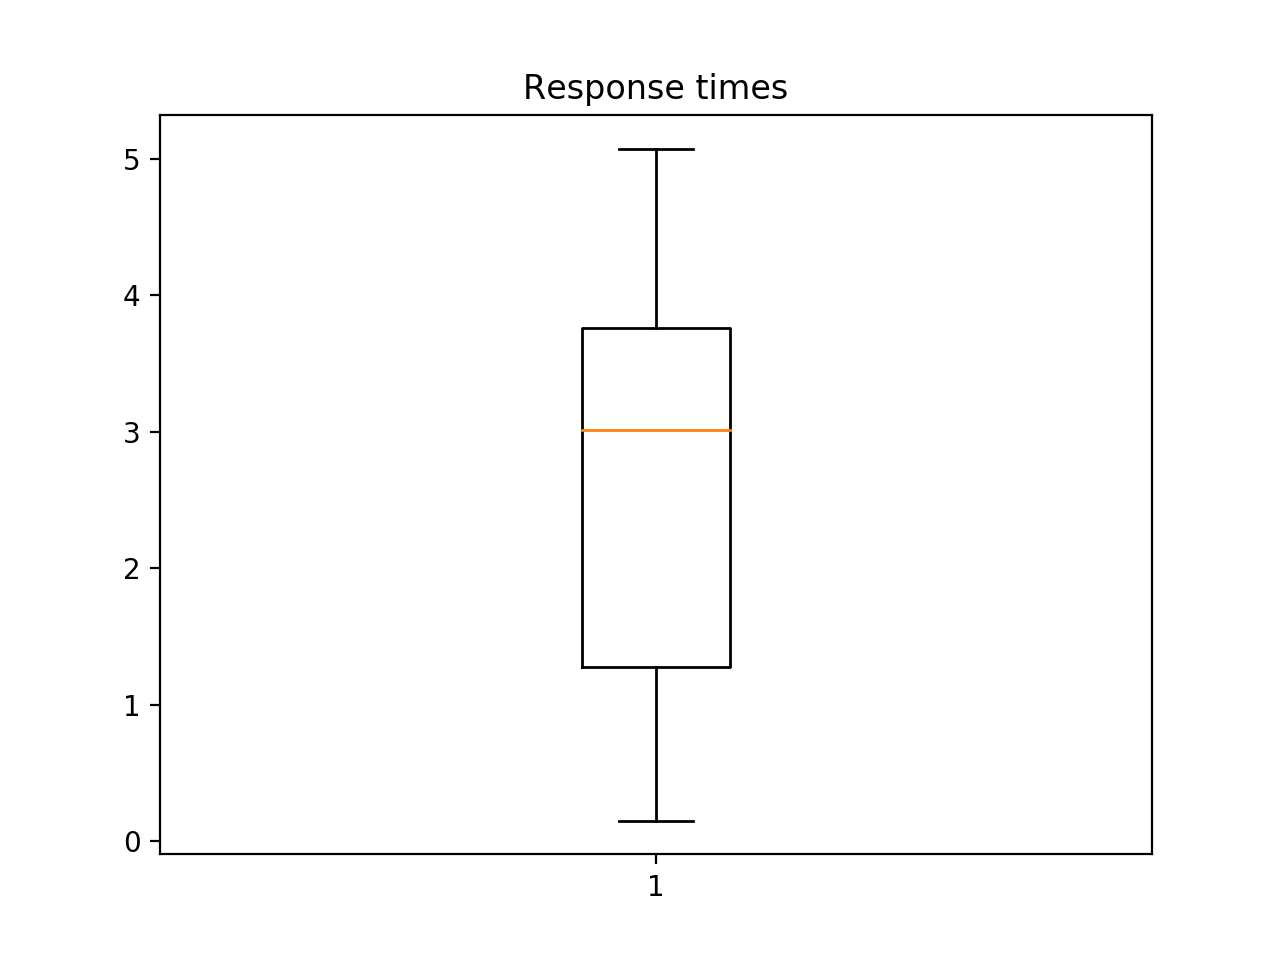
\includegraphics[scale=0.5]{diagrams/boxplot.png}
	\caption{\label{proofofconcept:boxplot}Response time from the proof of concept.}
	
\end{figure}

\newpage
\section{Can it be built?}
After considering the data gathered from our preliminary simulation in section 2 and the results obtained from the proof of concept in section 3, we belief that it is indeed possible to build a system that will meet the given requirements.

\section{Next steps}
In order to transform the proof of concept into an actual application, one would need to refine some details. For instance, the actual encryption and decryption of messages has been omitted due to the insignificant contribution to runtime they would have had. Due to testing reasons we omitted the limit on number of tickets that can be bought, this can easily be added by adding a counter to each user in the Users service for instance. An extra check on this counter should also be added.\\
The Service Level Agreements with different banking companies need to be negotiated in order to ensure the desired bank transaction times. Proven in \nameref{simulation} to be of minor importance, it is still advised to aim for a maximal waiting time of 5 seconds due to the results from \nameref{POC}. \\
We encourage anyone to see if any improvements can be made to further reduce the total time needed to process a request.

\newpage
\clearpage
\newpage
\begin{appendices}
	\section{Class diagram}
	\begin{figure}[h]
		\includegraphics*[scale=0.7]{diagrams/class-diagram.png}
	\end{figure}
	
	\clearpage
	\newpage
	
	\section{Deployment diagram}
	Generated by running following command in the folder containing the docker yml file: \\
	\texttt{docker run --rm -it --name dcv -v $``$(pwd):/input$"$ pmsipilot/docker-compose-viz}\\
	\begin{figure}[h]
		\includegraphics*[scale=0.3]{diagrams/docker-compose.png}
	\end{figure}
	
	\clearpage
	\newpage
	\section{Sequence diagrams}
	\subsection{Requirement 1: load balancing}
		\begin{figure}[h]
			\includegraphics*[scale=0.7]{diagrams/FR1.png}
		\end{figure}
	\clearpage
	\newpage
	\subsection{Requirement 2: encryption}
		\begin{figure}[h]
			\includegraphics*[scale=0.7]{diagrams/FR2.png}
		\end{figure}
	\clearpage
	\newpage
	\subsection{Requirement 3: balance check}
		\begin{figure}[h]
			\includegraphics*[scale=0.7]{diagrams/FR3.png}
		\end{figure}
	\clearpage
	\newpage
	\section{ABS code}
	\label{appendix:abscode}
	\begin{lstlisting}[language=json]
	// duration(x, y) means waiting at least x miliseconds and at most y miliseconds
	
	module TML;
	import * from ABS.DC;
	
	interface LoadBalancer {
	Unit addWorker(Shop s);
	Shop getWorker();
	Unit releaseWorker(Shop s);
	}
	
	class RoundRobinLoadBalancer() implements LoadBalancer {
	List<Shop> available = Nil; 
	List<Shop> inuse = Nil;
	
	Unit addWorker(Shop s){
	available = appendright(available,s);
	}
	
	Shop getWorker(){
	await (available != Nil);
	Shop s = head(available); 
	available = tail(available); 
	inuse = appendright(inuse,s);
	return s;
	}
	
	Unit releaseWorker(Shop s){
	available = appendright(available,s); 
	inuse = without(inuse,s);
	}
	
	}
	
	interface User {
	Bool register();
	Bool authenticate();
	Bool tickets();
	String getName();
	String getEmail();
	String getCCtype();
	}
	
	class User(String name, Int age, String cctype, String email, Keyvault k) implements User {
	Bool register() {
	await duration(10, 99/2);
	println("Registered " + name);
	return True;
	}
	
	Bool authenticate(){
	await duration(10, 59/2);
	return True;
	}
	
	Bool tickets(){
	await duration(30, 99/2);
	println("Printing tickets");
	return True;
	}
	
	String getName() {
	k.encrypt();
	return name;
	}
	
	String getEmail() {
	k.encrypt();
	return email;
	}
	
	String getCCtype() {
	k.encrypt();
	return cctype;
	}
	
	}
	
	interface Shop {
	Bool buyTickets(Int amount, User u, String date1, String date2);
	}
	
	class Shop(Bank b, Keyvault k, Tickets t, Duration responseTime) implements Shop {
	Bool buyTickets(Int amount, User u, String date1, String date2){
	Bool status = True;
	if (amount>4){
	println("Too many tickets ordered, abort");
	status = False;
	}
	
	Bool ticket_status = t.checkAvailable(date1, date2, amount);
	//println(toString(ticket_status));
	if (ticket_status == True){
	String cctype = await u!getCCtype();
	Bool temp = k.decrypt();
	Bool payment = await b!process(42, cctype);
	if (!payment){
	status = False;
	t!releaseTickets(date1, date2, amount);
	}
	else{
	println("Tickets have been successfully booked");
	}
	}
	else{
	println("No ticket available");
	status = False;
	}
	println(toString(now()));
	return status;
	}
	}
	
	interface Bank {
	Bool process(Int price, String cctype);
	}
	
	class Bank(Keyvault k) implements Bank {
	Bool process(Int price, String cctype){
	Bool status = True;
	if (cctype == "visa"){
	await duration(200, 800); 
	}
	else if (cctype == "maestro"){
	await duration(500, 1500);
	}
	else if (cctype == "mastercard"){
	await duration(100, 600);
	}
	return status;
	}
	}
	
	interface Keyvault {
	Bool encrypt();
	Bool decrypt();
	}
	
	class Keyvault() implements Keyvault {
	Bool encrypt(){
	await duration(40, 50);
	return True;
	}
	
	Bool decrypt(){
	await duration(40, 50);
	return True;
	}
	}
	
	interface Tickets {
	Bool checkAvailable(String date1, String date2, Int amount);
	Bool releaseTickets(String date1, String date2, Int amount);
	Bool addTickets(String date1, String date2, Int amount);
	}
	
	class Tickets() implements Tickets{
	Map<Pair<String, String>, Int> tickets = map[];
	
	Bool checkAvailable(String date1, String date2, Int amount){
	Bool status = True;
	Pair<String, String> period = Pair(date1, date2);
	Int available = lookupDefault(tickets, period, 0);
	if (amount >= available) {
	status = False;
	}
	else{
	Int temp = available;
	available = temp-amount;
	tickets = put(tickets, period, available);
	status = True;
	}
	return status;
	}
	
	Bool releaseTickets(String date1, String date2, Int amount){
	Pair<String, String> period = Pair(date1, date2);
	Int available = lookupDefault(tickets, period, 0);
	Int temp = available;
	available = temp+amount;
	tickets = put(tickets, period, available);
	return True;
	}
	
	Bool addTickets(String date1, String date2, Int amount){
	Pair<String, String> period = Pair(date1, date2);
	Pair<Pair<String, String>, Int> p = Pair(period, amount);
	tickets = insert(tickets, p);
	return True;
	}
	}
	
	{
	CloudProvider p = new CloudProvider("TML");
	await p!setInstanceDescriptions(
	map[Pair("T2_MICRO", map[Pair(Memory,1), Pair(Speed,1)]),
	Pair("T2_SMALL", map[Pair(Memory,2), Pair(Speed,1)]),
	Pair("T2_MEDIUM", map[Pair(Memory,4), Pair(Speed,2)]),
	Pair("M4_LARGE", map[Pair(Memory,8), Pair(Speed,2)])]);
	
	DC  server1 = await p!launchInstanceNamed("T2_SMALL");
	DC  server2 = await p!launchInstanceNamed("T2_SMALL");
	DC  server3 = await p!launchInstanceNamed("T2_SMALL");
	
	DC  server4 = await p!launchInstanceNamed("M4_LARGE");
	DC  server5 = await p!launchInstanceNamed("M4_LARGE");
	DC  server6 = await p!launchInstanceNamed("M4_LARGE");
	DC  server7 = await p!launchInstanceNamed("M4_LARGE");
	
	[DC: server4] Keyvault kv = new Keyvault();
	[DC: server5] Bank bank = new Bank(kv);
	[DC: server6] LoadBalancer lb = new RoundRobinLoadBalancer();
	[DC: server7] Tickets t = new Tickets();
	
	Int nmbrTickets = 10000000;	// This values can be changed for testing purposes
	t!addTickets("01-07-2020", "03-07-2020", nmbrTickets);
	
	Int nrWorkers = 100;
	while(nrWorkers > 0){
	Fut<DC> fs = p!launchInstanceNamed("M4_LARGE"); 
	DC vm = fs.get;
	[DC: vm] Shop shop = new Shop(bank, kv, t, Duration(1000));
	lb.addWorker(shop); 
	nrWorkers = nrWorkers-1;
	}
	
	Int nrJobs = 10000;	// Number can be changed for testing purposes
	println(toString(now()));
	while(nrJobs>0){
	Fut<Shop> s = lb!getWorker();
	User u = new User(toString(nrJobs), 22, "mastercard", "email", kv);
	Shop shopworker = s.get;
	shopworker!buyTickets(4, u, "01-07-2020", "03-07-2020");
	lb.releaseWorker(shopworker);
	nrJobs = nrJobs - 1;
	} 
	
	println(toString(now())); 
	println("DONE");
	}
	\end{lstlisting}
	
\end{appendices}

\begin{thebibliography}{00}
\bibitem{b1} Einar Broch Johnsen and Silvia Lizeth Tapia Tarifa, ``Modelling Auto-scalable Services Using Real Time ABS,'' https://abs-models.org/tutorial\_pdfs/scaling.pdf
\bibitem{b2} Einar Broch Johnsen, ``Modeling Deployment Decisions for Elastic Services with ABS,'' http://www.envisage-project.eu/modeling-deployment-decisions-for-elastic-services-with-abs/

\end{thebibliography}

\end{document}
